\chapter{Analiza sygnału}
Oryginalny sygnał wydobyty z nagrania został przedstawiony na spektrogramie (rys.~\ref{original}).

\begin{figure}
\centering
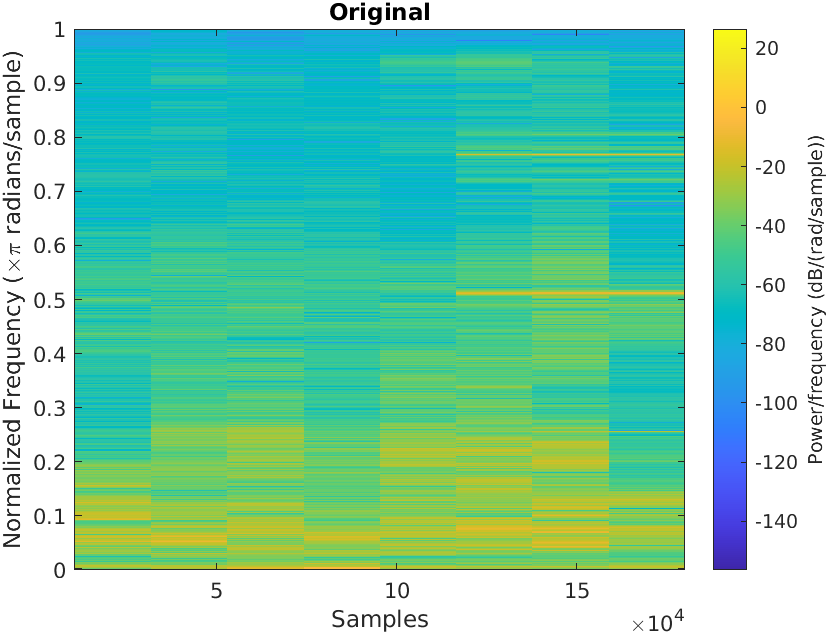
\includegraphics{dane/original.png} % [width=1\textwidth]
\caption{Spektrogram oryginalnego sygnału}
\label{original}
\end{figure}

Jak łatwo zauważyć, na całej długości sygnału znajduje się duże nagromadzenie niskich częstotliwości.
Jest to spowodowane obecnością szumu elektrycznego w~nagraniu.
Dodane przez niego częstotliwości są tak niskie, że można je spokojnie wyciąć nie przejmując się tym, czy zniekształci to ludzką mowę.

Kolejnymi ważnymi elementami spektrogramu~\ref{original} są dwie poziome kreski zaczynające się w~okolicy \num{110000}~-~\num{120000} próbek i~trwające do końca nagrania.
To one są odpowiedzialne za pojawianie się na nagraniu dźwięku budzika.
Jednak ponieważ pasma te są tak cienkie, to można je spokojnie wyciąć na całej długości nagrania.
Nie spowoduje to utraty jakichkolwiek części rozmowy.

\chapter{Filtry}

\section{Realizacja}

Do realizacji postawionego zadania musiały zostać stworzone filtry w dziedzinie częstotliwości.

Najpierw zaprogramowany został filtr dolnoprzepustowy.
Jego realizacja pozwala na dobranie własnej częstotliwości odcięcia podawanej w Hz, szerokości pasma przejściowego oraz typu okna wygładzającego przycięty filtr.
Filtr ten napisany został jako funkcja pakietu MATLAB, a jego kod wygląda następująco:

\begin{lstlisting}[style=Matlab-editor]
function low_pass = create_low_pass(fc, BW, fs)
fc = fc/fs;
M = 4 / BW;
t = (-M/2 : 1 : M/2);
t_moved = (0 : 1 : M);
h = (sin(2*pi*fc*t) ./ t);
h(M/2+1) = 2*pi*fc;
h = h / sum(h);
%% okno
window = "blackman";
hamming = 0.54 - 0.46 * cos(2*pi*t_moved/M);
blackman = 0.42 - 0.5 * cos(2*pi*t_moved/M) + 0.08 * cos(4*pi*t_moved/M);
if window == "hamming"
	low_pass = h .* hamming;
elseif window == "blackman"
	low_pass = h .* blackman;
end
end
\end{lstlisting}

Kolejne filtry tworzone są jako przekształcenie filtra dolnoprzepustowego.
Dlatego też kolejną funkcją wymagającą implementacji była inwersja spektralna filtra.
Kod tej funkcji został przedstawiony poniżej:

\begin{lstlisting}[style=Matlab-editor]
function new_kernel = inverse_filter(kernel)
new_kernel = -kernel;
new_kernel((length(kernel) - 1) / 2 + 1) = new_kernel((length(kernel) - 1) / 2 + 1) + 1;
end
\end{lstlisting}

Za pomocą tego filtra można łatwo z filtra dolnoprzepustowego stworzyć filtr górnoprzepustowy co zostało wykonane w poniższej funkcji \verb|create_high_pass|

\begin{lstlisting}[style=Matlab-editor]
function high_pass = create_high_pass(fc, BW, fs)
high_pass = inverse_filter(create_low_pass(fc, BW, fs));
end
\end{lstlisting}

Do pełnego wachlarza filtrów zostały tylko filtry pasmowo-blokujący oraz pasmowo-przepustowy.
Ich implementacja opiera się na tworzeniu, przekształcaniu i dodawaniu do siebie filtrów górnoprzepustowego i dolnoprzepustowego.
Pełna implementacja funkcji została przedstawiona poniżej dla filtra pasmowo-zaporowego:

\begin{lstlisting}[style=Matlab-editor]
function band_stop = create_band_stop(fc_low, fc_high, BW, fs)
low_pass = create_low_pass(fc_low, BW, fs);
high_pass = create_high_pass(fc_high, BW, fs);
band_stop = low_pass + high_pass;
end
\end{lstlisting}

Oraz pasmowo-przepustowego:

\begin{lstlisting}[style=Matlab-editor]
function band_pass = create_band_pass(fc_high, fc_low, BW, fs)
low_pass = create_low_pass(fc_low, BW, fs);
high_pass = create_high_pass(fc_high, BW, fs);
band_pass = conv(low_pass, high_pass);
end
\end{lstlisting}

%TODO zrobić charakterystykę amplitudową przygotowanych filtrów (wzmocnienie w dziedzinie częstotliwości)
\section{Weryfikacja}
Aby zobaczyć, czy stworzone filtry działają prawidłowo przeprowadzono kilka testów.
Wszystkie polegały na obserwacji wzmocnienia w dziedzinie częstotliwości.

Najpierw sprawdzono filtr górnoprzepustowy.
Eksperymenty polegały na ustawieniu takich samych parametrów poza szerokością pasma przejściowego.
Dla jednego filtra szerokość pasma przejściowego została ustawiona na \num{0.1}, czego wynik został przedstawiony na rys.~\ref{highpass01}, a dla drugiego na \num{0.005}, czego wynik można zobaczyć na rys.~\ref{highpass0005}.
Jak łatwo zauważyć częstotliwość odcięcia jest poprawnie odzwierciedlona na obu rysunkach, a szerokość pasma przejściowego również zachowuje się tak jak byśmy tego oczekiwali, czyli im większą wartość wstawimy, tym szersze jest to pasmo.

\begin{figure}
\centering
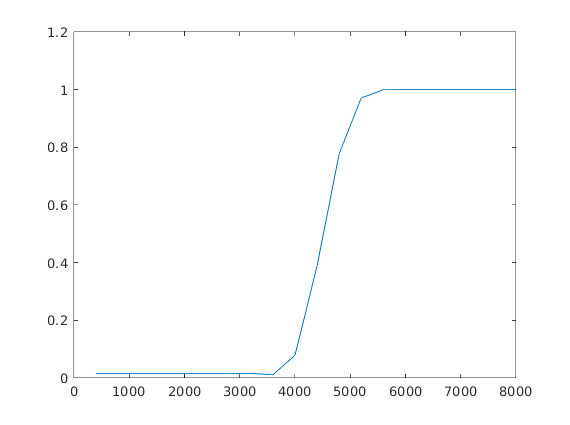
\includegraphics{dane/highpass01.png} % [width=1\textwidth]
\caption{Charakterystyka amplitudowa filtra górnoprzepustowego o częstotliwości odcięcia \num{4} kHz i szerokości pasma przejściowego \num{0.1}}
\label{highpass01}
\end{figure}

\begin{figure}
\centering
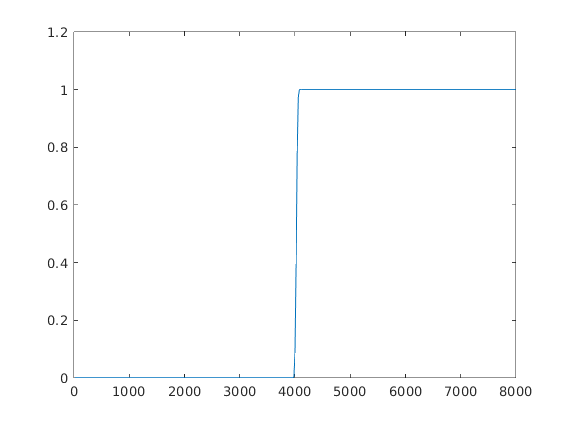
\includegraphics{dane/highpass0005.png} % [width=1\textwidth]
\caption{Charakterystyka amplitudowa filtra górnoprzepustowego o częstotliwości odcięcia \num{4} kHz i szerokości pasma przejściowego \num{0.005}}
\label{highpass0005}
\end{figure}

W kolejnym eksperymencie sprawdzono działanie filtra środkowo-zaporowego na takiej samej zasadzie jak górnoprzepustowego powyżej.
Oba filtry zostały ustawione na wycinanie częstotliwości z zakresu \num{4} kHz do \num{5} kHz.
Jeden posiadał pasmo przejściowe szerokości \num{0.05}, a drugi \num{0.005}.
Zostało to zaprezentowano odpowiednio na rys.~\ref{bandstop005} oraz rys.~\ref{bandstop0005}.
Jak widać, również w tym eksperymencie udowodniona została poprawność działania filtra.
Częstotliwości odcięcia zgadzają się z zadanymi, a szerokość pasma przejściowego zmienia się na rysunku odpowiednio do tego jaka została ustawiona.

\begin{figure}
\centering
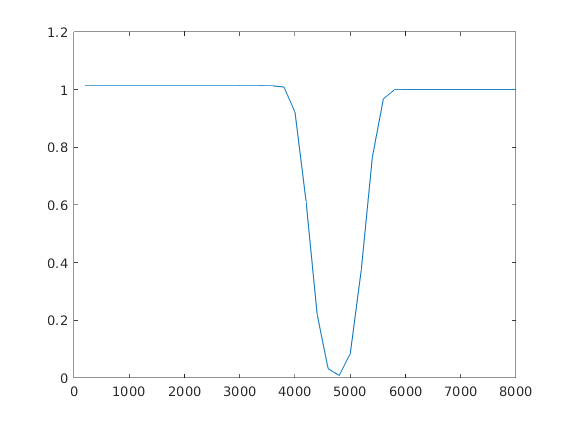
\includegraphics{dane/bandstop005.png} % [width=1\textwidth]
\caption{Charakterystyka amplitudowa filtra środkowo-zaporowego o częstotliwościach odcięcia \num{4} kHz i \num{5} kHz oraz szerokości pasma przejściowego \num{0.05}}
\label{bandstop005}
\end{figure}

\begin{figure}
\centering
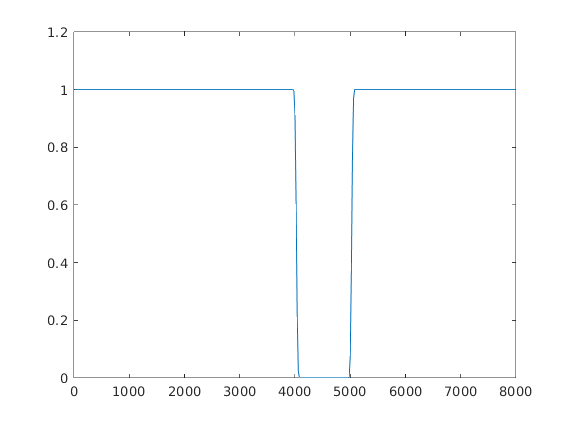
\includegraphics{dane/bandstop0005.png} % [width=1\textwidth]
\caption{Charakterystyka amplitudowa filtra środkowo-zaporowego o częstotliwościach odcięcia \num{4} kHz i \num{5} kHz oraz szerokości pasma przejściowego \num{0.005}}
\label{bandstop0005}
\end{figure}

Kolejnych eksperymentów nie było sensu przeprowadzać, ponieważ pozostałe filtry opierają się na przekształceniach tych opisanych powyżej, więc jeżeli te działają, to pozostałe również powinny.

\chapter{Wyniki}
Tak jak zostało to przedstawione w części z analizą sygnału, za pomocą filtra pasmowo~-~zatrzymującego, zostały wycięte dwa bardzo wąskie pasma częstotliwości: jedno od \num{4000} Hz do \num{4250} Hz, a drugie od \num{6000} Hz do \num{6250} Hz.
Te dwa pasma były odpowiedzialne za najbardziej słyszalną część dzwonienia budzika.
Następnie odfiltrowano, filtrem górnoprzepustowym, wszystko co znajdowało się poniżej \num{200} Hz.
W ten sposób udało się praktycznie całkowicie zlikwidować dźwięk zakłócenia sieciowego z nagrania.

Kod skryptu dokonującego tych wszystkich operacji w programie MATLAB został przedstawiony poniżej:

\begin{lstlisting}[style=Matlab-editor]
%% wczytywanie sygnalu
[x, fs] = audioread("noised.wav");
%% parametry filtrow
BW = 0.005;
%% filtracja sygnalu
sig = x;
sig = conv(sig, create_band_stop(6000, 6250, BW, fs));
sig = conv(sig, create_band_stop(4000, 4250, BW, fs));
sig = conv(sig, create_high_pass(200, BW, fs));
%% spektrogramy
subplot(1, 2, 1); spectrogram(x, 'yaxis'); title('Original');
subplot(1, 2, 2); spectrogram(sig, 'yaxis'); title('Filtered');
%% zapisanie sygnalu i odsluchanie
% audiowrite("denoised.wav", sig, fs);
sound(sig, fs);
\end{lstlisting}

Spektrogram sygnału po filtracji pokazany został na rys.~\ref{filtered}

\begin{figure}
\centering
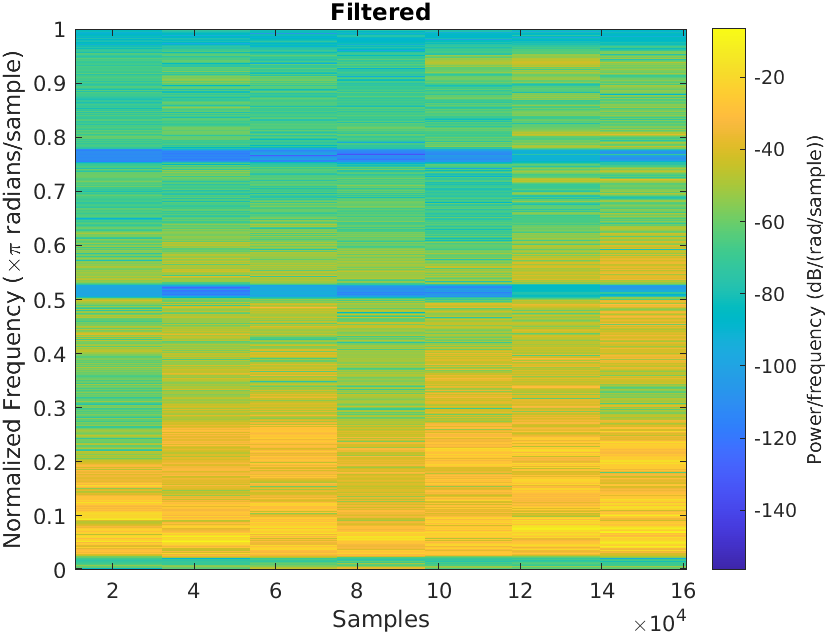
\includegraphics{dane/filtered.png} % [width=1\textwidth]
\caption{Spektrogram sygnału po odfiltrowaniu zakłóceń}
\label{filtered}
\end{figure}

\section{Subiektywna ocena wyników}
Podczas dobierania filtrów szczególną uwagę zwrócono na to, aby nie zniekształcić rozmowy.
Dlatego też podczas odsłuchiwania wyniku filtracji można usłyszeć ciągle słabe szumienie sprzężenia sieciowego oraz lekki przydźwięk od budzika.
Nie są to jednak rzeczy które przeszkadzają, sygnał został znacznie oczyszczony i rozmowa jest słyszalna zdecydowanie wyraźniej.
Oznacza to, że cel został osiągnięty.
